\nonstopmode
\documentclass{beamer}
\usepackage[utf8]{inputenc}
% \usepackage[frenchb]{babel}
\usepackage{amsmath}
\usepackage{mathtools}
\usetheme{Luebeck}
\useoutertheme[footline=authortitle,subsection=false]{miniframes}

\usepackage{tabu}
\usepackage{multicol}
\usepackage{vwcol}
\usepackage{stmaryrd}
\usepackage{graphicx}

\title{Classification of Sleep Phases with EEG and Accelerometer Data}
\subtitle{Challenge Data -- Dreem}
\author{Alex AUVOLAT}
\date{Febuary 24, 2016}

\begin{document}

\begin{frame}
\titlepage
\end{frame}

\begin{frame}
\frametitle{Overview}
\tableofcontents
\end{frame}

\section{Task Presentation}
\frame{\sectionpage}

\begin{frame}
	\frametitle{Dataset characteristics}
	\begin{itemize}
		\item 31129 training points
		\item 30458 test points
	\end{itemize}
	Features:
	\begin{itemize}
		\item 15 seconds of EEG data, 250 Hz, 1 channel $\to$ 3750 values
		\item 15 seconds of accelerometer data, 10 Hz, 3 channels $\to$ 350 values
	\end{itemize}
\end{frame}

\begin{frame}
	\frametitle{Signal categories}
	\begin{table}\centering
	\begin{tabular}{l l l l}
		\textbf{Class}&\textbf{Code}&\textbf{Description}&\textbf{Count}\\ \hline
		0 & & Wake & 1342\\
		1 & N1 & Light sleep ("somnolence") & 428 \\
		2 & N2 & Intermediate sleep & 15334 \\
		3 & N3 & Deep sleep & 9640 \\
		4 & REM & Paradoxical sleep & 4385 \\ \hline
		& & \textbf{Total} & 31129 \\
	\end{tabular}
	\end{table}
\end{frame}

\begin{frame}
	\frametitle{Typical EEG signal (REM sleep)}
	\begin{figure}
		\centering
		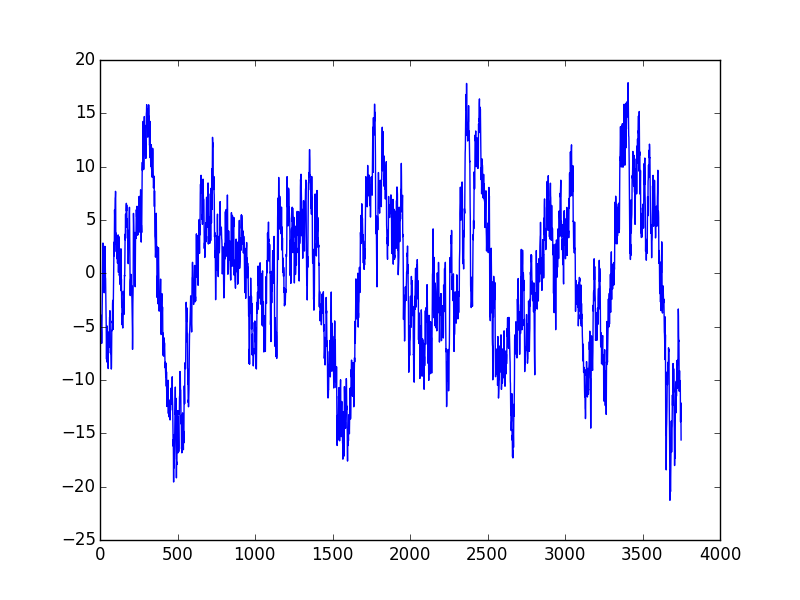
\includegraphics[width=10cm]{../typical_eeg_REM.png}
	\end{figure}
\end{frame}

\begin{frame}
	\frametitle{Typical ACC signal (N2 sleep)}
	\begin{figure}
		\centering
		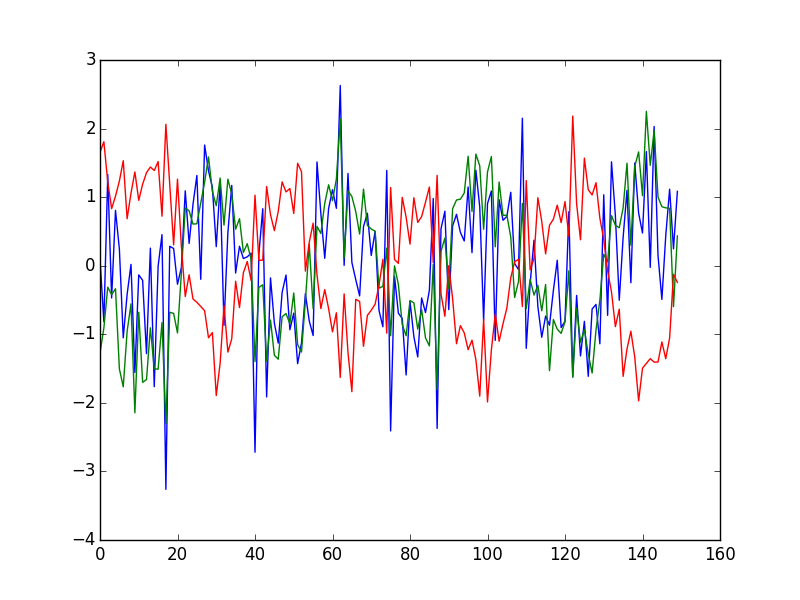
\includegraphics[width=10cm]{../typical_acc_2_N2.png}
	\end{figure}
\end{frame}

\section{Feature Extraction}
\frame{\sectionpage}

\begin{frame}
	\frametitle{Wavelet transform}
	We first convolve the signal with a series of Ricker wavelets:
	$$\psi_\sigma(t) = {2 \over {\sqrt {3\sigma}\pi^{1 \over 4}}} \left( 1 - {t^2 \over \sigma^2} \right) e^{-t^2 \over 2\sigma^2}$$

	The values of $\sigma$ are spaced regularly on a logarithmic scale:

	$$\sigma_i = 2^i$$
	$$\sigma_0 = 1$$
	$$\sigma_{10} = 1024$$
\end{frame}

\begin{frame}
	\frametitle{Wavelets}
	\begin{figure}
		\centering
		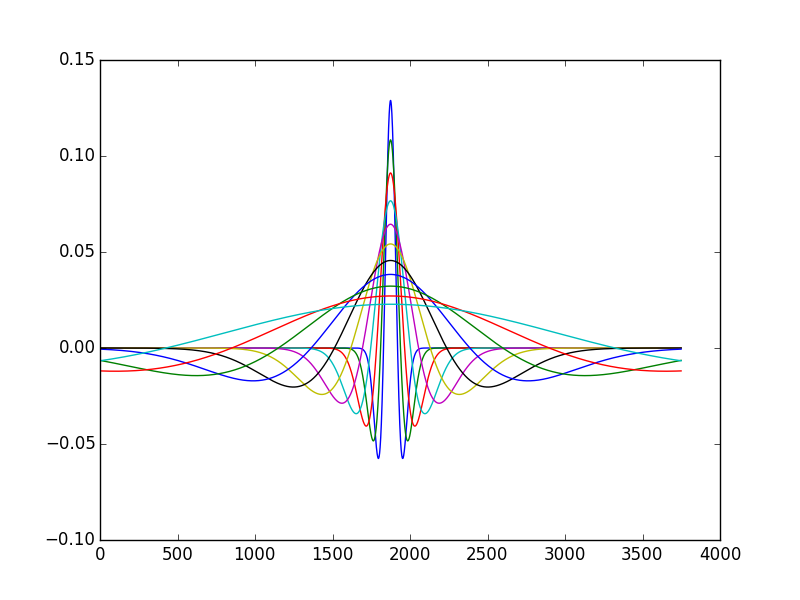
\includegraphics[width=10cm]{../half_wavelets.png}
	\end{figure}
\end{frame}

\begin{frame}
	\frametitle{Wavelets, in the Fourier domain}
	\begin{figure}
		\centering
		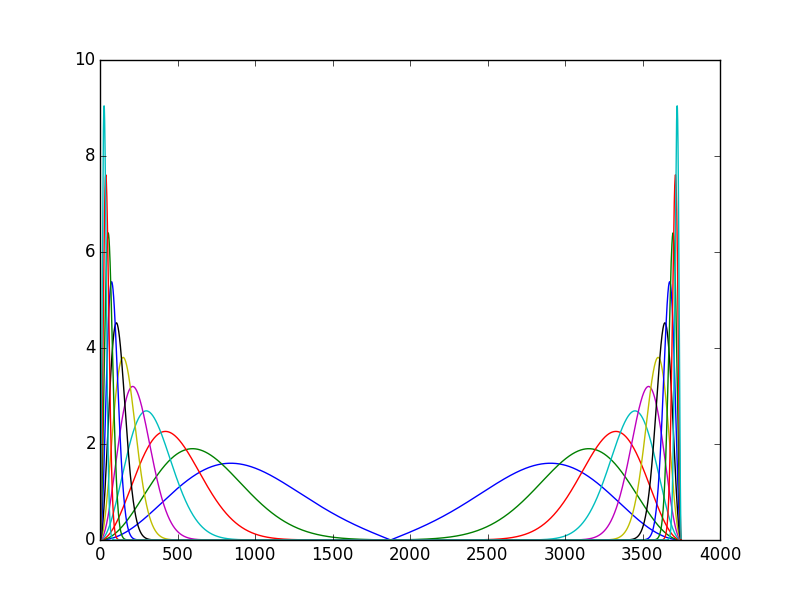
\includegraphics[width=10cm]{../half_wavelets_fft.png}
	\end{figure}
\end{frame}

\begin{frame}
	\frametitle{Remarks}
	Convolution is equivalent to a multiplication in the Fourier domain, which has several implications:
	\begin{itemize}
		\item convolution can be done very quickly
		\item we can interpret the convolution by a wavelet as exacerbating certain frequency range while extinguishing others
	\end{itemize}
\end{frame}

\begin{frame}
	\frametitle{Our signal (EEG), in the Fourier domain}
	\begin{figure}
		\centering
		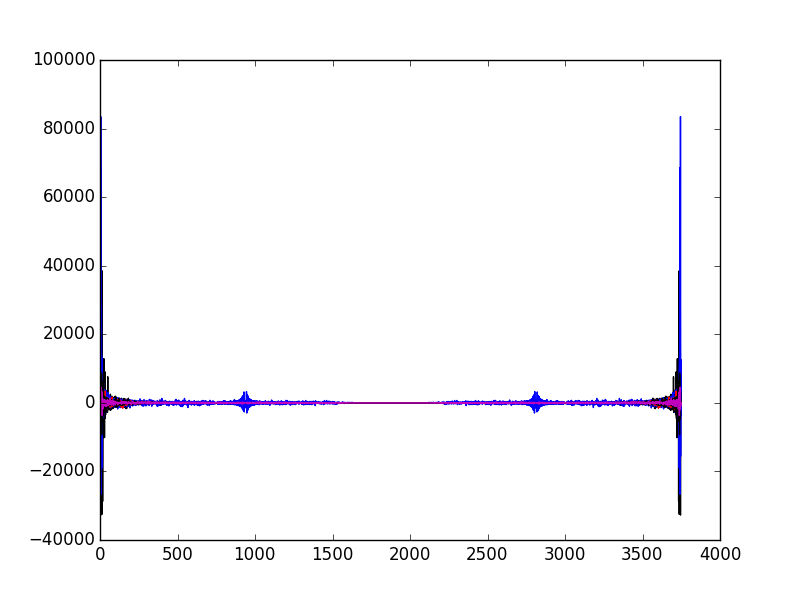
\includegraphics[width=10cm]{../__fft_eeg.png}
	\end{figure}
\end{frame}

\begin{frame}
	\frametitle{Now, convolved with a high-frequency wavelet ($\sigma=1$)}
	\begin{figure}
		\centering
		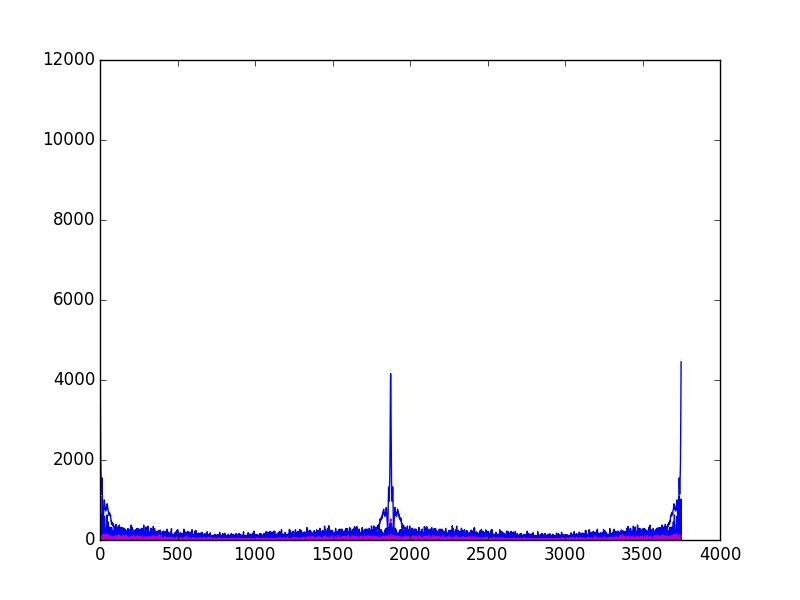
\includegraphics[width=10cm]{../__sig1_eeg_0.png}
	\end{figure}
\end{frame}

\begin{frame}
	\frametitle{With a lower frequency ($\sigma=4$)}
	\begin{figure}
		\centering
		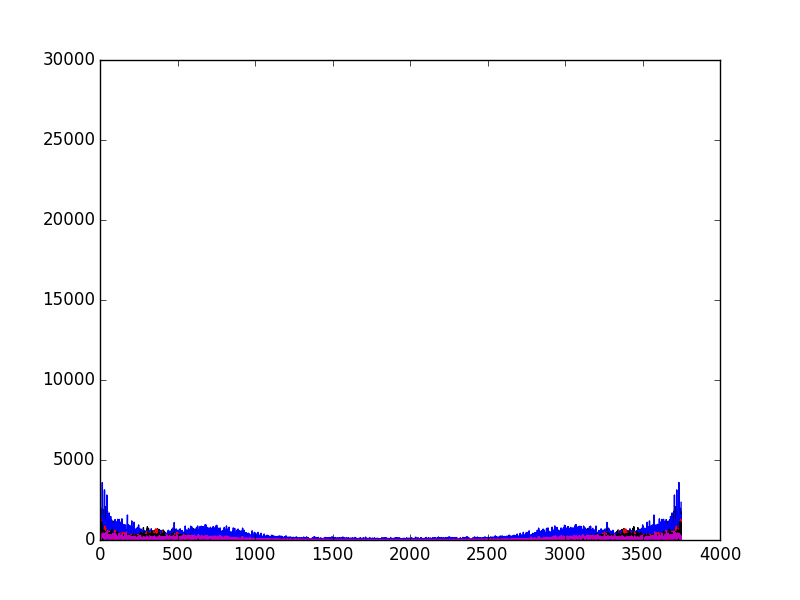
\includegraphics[width=10cm]{../__sig1_eeg_1.png}
	\end{figure}
\end{frame}

\begin{frame}
	\frametitle{With an even lower frequency ($\sigma=16$)}
	\begin{figure}
		\centering
		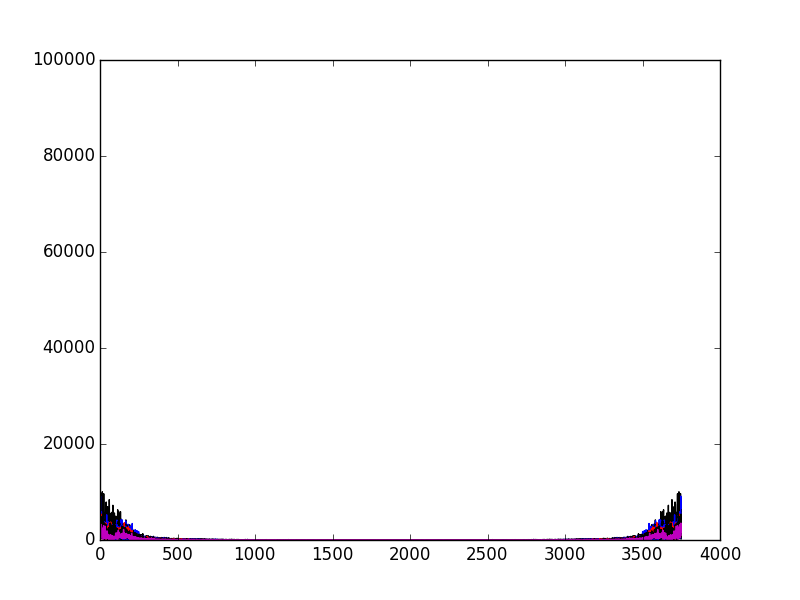
\includegraphics[width=10cm]{../__sig1_eeg_2.png}
	\end{figure}
\end{frame}

\begin{frame}
	\frametitle{Dimensionality reduction}
	\begin{itemize}
		\item It is impossible to run a classifier on $11\times3750$ features for $30000$ examples.
		\item We use a PCA to transform the $3750$-dimensional signal into a $15$-dimensional signal.
		\item For the EEG, we end with $15\times11=165$ features
		\item Similar processing for the accelerometer data.
	\end{itemize}
\end{frame}

\begin{frame}
	\frametitle{Feature vectors}
	\begin{figure}
		\centering
		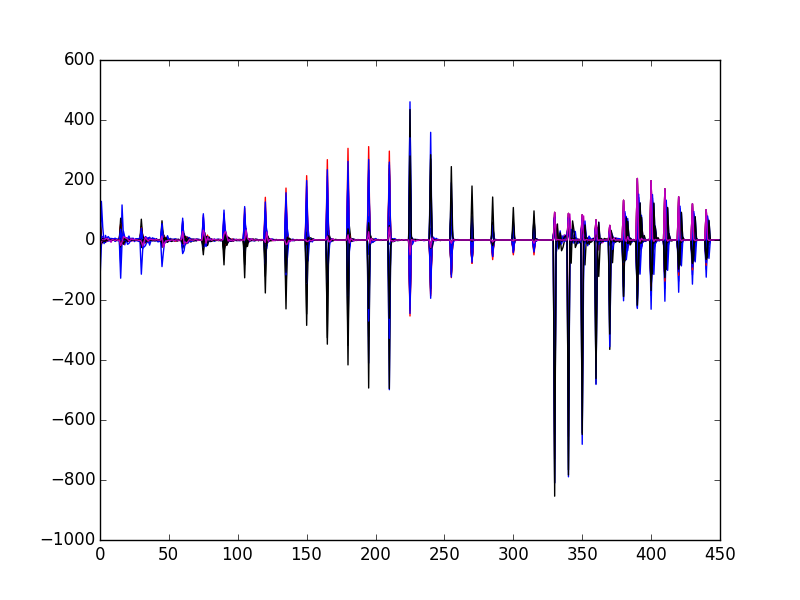
\includegraphics[width=10cm]{../model50/__features.png}
	\end{figure}
\end{frame}

\section{Classification & Results}
\frame{\sectionpage}

\begin{frame}
	\frametitle{Random Forest Classification}
	\begin{itemize}
		\item Classification is done with a random forest
		\item Parallel implementation provided by \texttt{scikit-learn}
		\item Tried using up to 128 trees to improve model performance (more trees improves the performance a little)
	\end{itemize}
\end{frame}

\begin{frame}
	\frametitle{Random Forest vs. Linear Classifiers}
	Random forest classifiers worked much better than linear classifiers on this task:
	\begin{itemize}
		\item Linear classifiers are much slower to train
		\item The problem is not completely linearly separable in our feature space
		\item Error rate: 22\% (linear classifier) vs. 15\% (random forest)
	\end{itemize}
\end{frame}

\begin{frame}
	\frametitle{Results}
	\begin{figure}
		\centering
		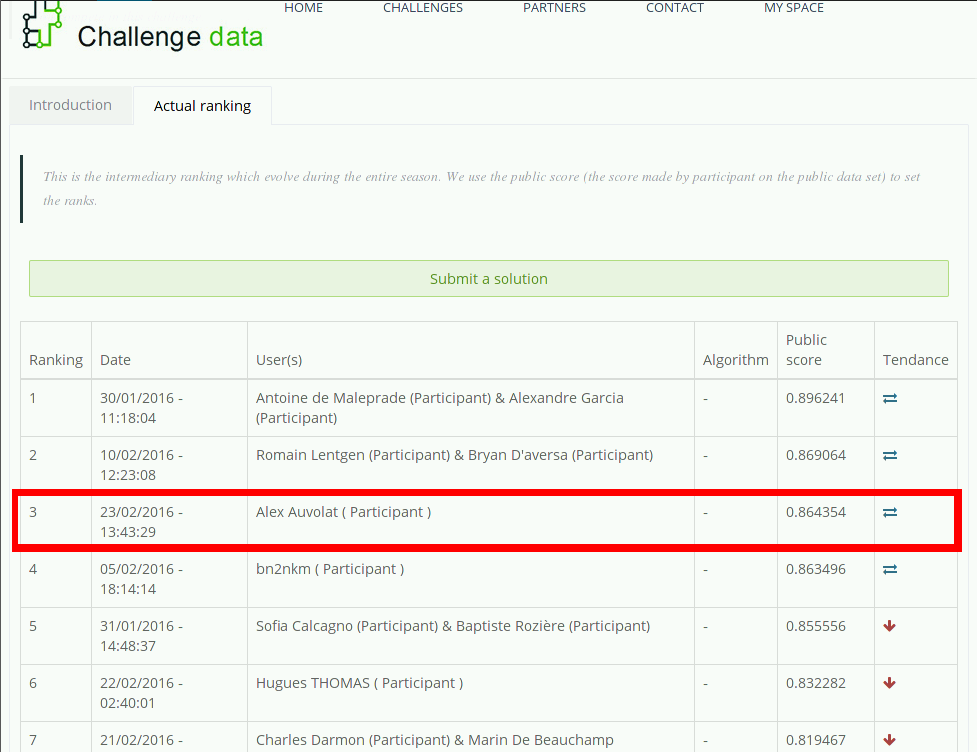
\includegraphics[width=9cm]{../CLASSMENT.png}
	\end{figure}
\end{frame}

\begin{frame}
	\frametitle{Remarks}
	\begin{itemize}
		\item Tried many variants, validating them on a subset of the training set, for local validation
		\item Results on the public leaderboard were usually far worse than on the validation set\\
		$\to$ overfitting...
		\item The best score I got on the leaderboard was actually with one of the first variants I tried

	\end{itemize}
\end{frame}


\end{document}

%% vim: set ts=4 sw=4 tw=0 noet spelllang=fr :
